\documentclass[10pt,twocolumn]{article}

% use the oxycomps style file
\usepackage{oxycomps}

% usage: \fixme[comments describing issue]{text to be fixed}
% define \fixme as not doing anything special
\newcommand{\fixme}[2][]{#2}
% overwrite it so it shows up as red
\renewcommand{\fixme}[2][]{\textcolor{red}{#2}}
% overwrite it again so related text shows as footnotes
%\renewcommand{\fixme}[2][]{\textcolor{red}{#2\footnote{#1}}}

% read references.bib for the bibtex data
\bibliography{references}

% include metadata in the generated pdf file
\pdfinfo{
    /Title (Using Robotics To Make Blinds Smarter)
    /Author (Maryo Botros)
}

% set the title and author information
\title{Using Robotics To Make Blinds Smarter}
\author{Maryo Botros}
\affiliation{Occidental College}
\email{mbotros@oxy.edu}

\begin{document}

\maketitle

\section{Introduction and Problem Context}

Smart home technology has been developing rapidly, and many consumers have felt compelled to adopt this technology into their homes to help improve their way of living. This has especially been the case since the onslaught of the Covid-19 pandemic, when people have started to spend more time at home \cite{Ghosh2021SmartHomeDevice}. Examples of these tools include smart locks that can lock and unlock based on the user's location and smart lights that can turn on and off depending on whether or not a person is detected in a room. These devices often use automation in some capacity, to perform the tasks that humans normally would and are meant to enhance a user’s experience, while still fundamentally functioning the same way.

Although this technology has gained more widespread adoption, there are still some areas of smart home technology that have yet to see development, namely, window blinds There are currently no mainstream smart home technology manufacturers that produce automated window blinds and yet blinds have great potential for improvement with automation. Blinds may seem simple because they are either opened or closed, but the ways people interact with them can be quite nuanced and reveal that automating blinds can bring significant improvements. Firstly, blinds can be automated to function as natural alarm clocks, automatically opening when the sun comes up. They can also be automated to automatically close when the sun sets, functioning as a privacy tool, as this is a time when people outside can see through a window. They can be automated to close at high temperatures to keep indoor temperatures cooler, which can save energy. Automated blinds can also allow a user to monitor their blinds remotely from an app, offering peace of mind. Additionally, automated blinds can be beneficial as an accessibility tool for users, especially those with disabilities who may have difficulties adjusting blinds according to their needs. Based on all of these use cases, there does exist a need for automating blinds.

The goal of this project is to automate blinds, using robotics. In order to do this, a robot that uses sensors and a motor will be needed to get readings on stimuli in the environment such as light and temperature, and then affect the blinds in response. A website will also be needed to allow the user to view the status of the blinds remotely and give the user the option for setting different modes and settings for the robot. This paper discusses the process for creating a robot that automates blinds along with the website that will pair with it. This process involves developing the robot and website and conducting two rounds of user testing to improve it. In the end, an evaluation is conducted to assess the success of the project, by testing the functions of the robot and gauging users’ experience testing it out.


\section{Technical Background}
\subsection{Smart Home Technology and Blinds}
Smart Home is the integration of technology and services through home networking for a better quality of living \cite{Hayes2022SmartHome}. These are devices that can cover many aspects of a home such as lighting, security, and heating, to name a few. Some smart locks, for example, are able to lock and unlock as a user walks up to a door. Often these smart home devices have some sort of app that allows a user to adjust settings or remotely interact with the smart home device in some way over an internet connection. Smart locks for example allow the user to lock and unlock a door remotely. These devices are meant to make the lives of a user better rather than more complicated. They should enhance a user’s life by making tasks more efficient or increasing accessibility without fundamentally changing the way they interact with a device or appliance \cite{Tamayo2022SmartHome}. It does not necessarily need to solve a problem but rather decreases the friction experience when doing everyday mundane tasks \cite{Tamayo2022SmartHome}.

There are many popular smart home devices such as security cameras, locks, and thermostats, however, one area of a smart home that currently lacks development is window blinds. In the year 2021, smart blinds did not appear on any list of the most popular smart home devices \cite{Woodall2021Popular}. Consumers are clearly interested in automating the tools and appliances they use at home and the lack of development with automated blinds, therefore, suggests that there have not been any compelling options offered yet.

Automated blinds currently have a lot of potential and many possible use cases. Automated blinds can serve as natural alarm clocks, automatically letting sunlight in a room as soon as the sun rises. They can be used as privacy devices, automatically closing when the sun goes down, which is the time when people usually turn lights on in the home and this would therefore compromise privacy as the indoors could be seen from the outside. Because of these two use cases, one way the blinds could be automated is by sensing light, opening when sunlight is detected, and shutting when it is not. Additionally, automated blinds can be closed when temperatures outside get too high, which would help keep indoor temperatures lower. This could also help reduce the amount of energy used for cooling down a room. Keeping a house cooler can significantly decrease the cost of energy and this could have even greater implications for commercial buildings that have dozens or hundreds of windows. Automated blinds can also offer a user peace of mind as the user can view the status of the robot and see whether the blinds are open or closed, remotely from an app. A use case for this could be if a user is not at home and wants to see if they made sure to shut the blinds before they left home. Although having blinds opened when not at home may not pose as great of a problem as leaving a door unlocked, for instance, it can still potentially be a security or privacy issue. Finally, automated blinds could function as an accessibility tool, especially for people who may suffer from disabilities, as they make it less necessary for a user to open and close the blinds manually, on their own.

In order to serve all of these use cases, a robot as well as an accompanying web application will be necessary. The web application will be needed to allow the user to see the status of the blinds as well as select between varying modes that use either light or temperature to automate the blinds. The robot, which will be called the blinds robot for the purpose of this paper, will be a device that can be retrofitted on a set of blinds. This robot will be able to sense light and temperature levels and use a motor to move the blinds. For the purpose of this project, no mechanical parts will be developed to physically attach the motor to the blinds as that is beyond the scope of this project.

\subsection{Project Architecture}
The robot for this project will be developed using an Arduino microcontroller. Arduino is an open-source hardware and software company and they manufacture the controller for the robot, which is like the brain of the robot and will be discussed later in this section. The robot will need to be able to communicate with the web application and there is no way to directly communicate between an Arduino and a web page interface, but it is possible to facilitate a connection between them is using a Node.js server that will pass messages back and forth \cite{Thomas2020Communicating}. In order to display the status of the robot, there needs to be a way to pass information from the Arduino to the webpage. Additionally, in order to select different modes so that the user can choose between what sensors they want to use on the Arduino, from the webpage, there needs to be a way to pass information from the webpage to the Arduino. The way these two processes will work is shown in Figure 1. The webpage will send information  back and forth with Node.js using socket.io and the Arduino will send information back and forth with Node.js using serialport. Socket.io is a library that enables real-time, bi-directional communication between clients and servers and serialport is a serial communication interface used in Arduino \cite{Fitzgerald2015Arduino}.

\begin{figure}
    \centering
    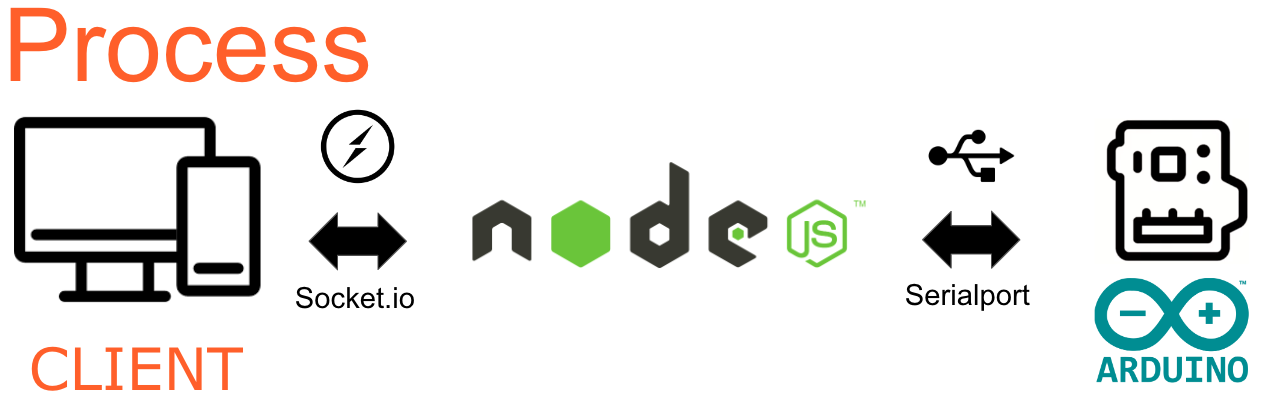
\includegraphics[width=.95\linewidth]{Figure 1.png}
    \caption{
        Architecture overview for the project.
    }
    \label{fig:first-page}
\end{figure}

\subsection{Robot}
The robot is a major component of this project, so it is important to understand robotics. Robotics is a quickly evolving field whose definition has been changing over time. A lot of the time, when people think of robots, they imagine metal, human-like machines trying to do human tasks. Although they don’t usually come in this form factor, oftentimes they are created to do menial tasks in the place of humans. Computer scientist and roboticist, Maja Mataric defines a robot as an autonomous system that exists in the physical world, can sense its environment, and can act on it to achieve some goals \cite{Mataric2007TheRoboticsPrimer}. Although Mataric’s definition is quite broad, it succinctly encompasses all of the important and necessary qualifications for what makes something a robot and it can be broken down into a few key requirements. 

\subsubsection{Physical}
The first requirement for a robot is that it must fundamentally exist in a physical world, meaning that it has to deal with the unbendable physical laws and challenges of the physical world. Having a physical body is known as embodiment \cite{Mataric2007TheRoboticsPrimer}. According to Mataric, this is what makes robots a real challenge and why robots that exist on a computer are simulations and not true robots because simulations are never as complex as the real world. The blinds robot is a physical thing because it has a body that is composed of all the components and it has to physically affect the blinds.

\subsubsection{Actuators and Effectors}
The robot has to exist in a physical world because it needs to affect the physical world and the way it does this is through actuators and effectors. Mataric likens effectors to legs, flippers, wings, and various other body parts that allow animals to move \cite{Mataric2007TheRoboticsPrimer}. These effectors use underlying mechanisms such as muscles and motors. These motors are referred to as actuators. Effectors are the parts of the robot that physically interact with its environment and the actuators are the muscles that power those effectors to move. For the blinds robot, the effector is the part of the servo motor that is attached to the blinds. The actuator is the servo motor, which is a type of geared motor that can only rotate 180 degrees \cite{Fitzgerald2015Arduino}. It is controlled by sending electrical pulses from the Arduino which tell it what position to move to \cite{Fitzgerald2015Arduino}.

\subsubsection{Sensors}
In order to perform any actions in the physical world, robots need to have an understanding of that physical world so that they can perform the appropriate actions and this is what sensors are for. Robots use sensors to perceive their environment and get information and they can then process and perform actions on this information. Mataric suggests that if a system does not sense or get information, then it is not a robot, because it cannot respond to what goes on around it \cite{Mataric2007TheRoboticsPrimer}. Mataric defines sensors as devices that allow the robot to perceive its physical environment to get information about itself and its surroundings \cite{Mataric2007TheRoboticsPrimer}. The terms sensing and perception are used interchangeably in robotics, both referring to the processes of receiving information about the environment through the use of sensors. The blinds robot will need to be able to sense temperature and light levels in order to affect the blinds. In order to sense temperature, a tmp36 sensor will be used and in order to sense light levels, a phototransistor will be used.

\subsubsection{Controller and Autonomy}
A robot can use its sensors to perceive the environment and it can then act on what it perceives using its actuators and effectors, but only if it has some way of processing the information that the sensors provide and only if it has a way of telling the actuators to affect the environment in a specific way. In order to accomplish this, the robot needs to have a controller. Controllers provide the hardware and/or software that makes the robot autonomous by using the sensor inputs to decide what actions to take and then to control the effectors to execute that action \cite{Mataric2007TheRoboticsPrimer}. They play the role of the brain in the entire operation and the controller for the blinds robot is an Arduino Uno microcontroller. This microcontroller is a simple computer and it is what uses its programming to then function autonomously. Mataric highlights that a robot is an autonomous system meaning that it acts on the basis of its own decisions, and is not controlled by a human \cite{Mataric2007TheRoboticsPrimer}. Although the blinds robot will need some user input from the webpage such as which mode it should use, it overall works autonomously, detecting sunlight and temperature levels, processing the information, and then taking appropriate actions, without any human intervention.

\subsubsection{Achieving Goals}
A true robot must act autonomously and exist physically to sense its environment, in order to accomplish goals. According to Mataric, we expect a true robot to have one or more goals and to act so as to achieve those goals \cite{Mataric2007TheRoboticsPrimer}. The goal of the blinds robot is to perform according to the mode it is set in. For example, if it is in the temperature mode, its goal is to get temperature readings, and then if that temperature is above a certain threshold, the robot should close the blinds, otherwise, it should open them.


\section{Prior Work}
\subsection{Overview}
Although there are no mainstream smart home manufacturers offering blinds that are automated, there are still some projects that are similar to this one in some capacity. Three examples of prior work that will be discussed are motorized blinds, SwitchBot’s Blind Tilt, and an Arduino smart home light switch controller. 

\subsection{Motorized blinds}
The most popular products that share similarities with the blinds that were created for this project are motorized blinds. Several companies manufacture these blinds and often advertise them as “smart blinds.”Smart blinds are window coverings that can be opened or closed through an app or a voice command on your smartphone. They come in various styles, such as accordion, slat, honeycomb, roller, and light filtering \cite{Alina20228BestSmartBlinds}. These blinds would not be considered robots because they do not use any sensors and so they are not automated in any way, which sets them apart from this project, as the focus of this project is controlling blinds in an automated fashion. Additionally, these products are the complete blinds set, whereas this project focuses on a robot that can be attached to any existing set of blinds to retrofit them. Where motorized blinds share some similarities with this project is that they both have some sort of way to connect to the blinds over the internet. The motorized blinds can be set to open or close from an app on a smartphone and for this project, the blinds can also be set to open or close from the website.

\subsection{SwitchBot Blind Tilt}
The project that shares the most similarities to this one is a blind titling robot that is made by a company called SwitchBot and is currently on Kickstarter. SwitchBot is a company that manufactures smart home technology at affordable prices, to make home appliances more interactive and fun \cite{SwitchBot2022}. The device is a robot that can be used to sense sunlight to open and close blinds and is attached to the wand of horizontal blinds \cite{WonderTechLab2022SwitchBot}. The device is powered using a solar panel and can be controlled to open and close from an app. A user can also use smart home assistants such as Amazon’s Alexa, Google Home, and Siri \cite{WonderTechLab2022SwitchBot}. There are a lot of similarities between this project and SwitchBot’s blind tilt. They are both robots that use sensors, specifically to measure sunlight to affect the blinds. They are also both built to be retrofitted on already existing blinds. Additionally, they both have some way of communicating with the robot over an internet connection. SwitchBot has an app that is associated with the device and for this project, there is a website that connects with the robot. A difference between their two interfaces for interacting with their robots is that SwitchBot’s app allows the user to set schedules for opening and closing the blinds, while the website for this project does not incorporate any scheduling feature. Another difference between this project and SwitchBot’s Blind Tilt is that SwitchBot’s Blind Tilt only uses a sensor that detects light, meanwhile for this project, there are other sensors that are employed such as a temperature sensor and a potentiometer, which additionally allows the user to employ a combination of light and temperature sensors in automating the blinds from the website, which Blind Tilt does not offer. 

\subsection{Arduino Remote Control Light Switch}
There are many similar smart home-related projects that others have made using Arduino, one of which is a remote-controlled light switch made. The Remote Control Light Switch is a device that mounts over an existing light switch and uses a servo motor to turn the light switch on and off \cite{MerrittRemoteControlLightSwitch}. A pair of radio transceivers, one in the device itself and one in the remote allow the user to control the light remotely \cite{MerrittRemoteControlLightSwitch}. Like this project, the Arduino remote Control Light Switch is a device that is created using an Arduino microcontroller and it is created to retrofit an already existing appliance or tool; the remote control light switch is built to be placed on a light switch and the robot for this project is built to attach to the wand of a set of blinds. They both also give users the ability to remotely interact with the appliance, albeit in different fashions. The light switch can be remotely controlled using a button on another Arduino, meanwhile, the robot for this project can be remotely controlled from a website. Another difference is that the remote control light switch is not a robot because it is not automated in any way.


\section{Methods}

\subsection{Sending Data From Arduino to Webpage}

The goal of the first milestone is to successfully get Arduino to communicate with the frontend and then also program the Arduino to control a servo motor based on the amount of light that it receives. My first step is finding a way to get the Arduino to communicate with the frontend. After researching the different ways to accomplish this, I found that running the entire process through a Nodejs server would give me the best chance at success. The process for how the Arduino is able to communicate with the frontend through the Nodejs server is outlined in Figure 1. The Arduino sends and receives data to and from the server through the serialport. The frontend sends and receives data to and from the server through websockets. In this first case my plan is to write a program for the Arduino where I will activate a switch on the Arduino and when this switch is activated, it should change the color of a square on the webpage.

The other goal is


Beyond the basic syntax, much of learning LaTeX is learning the different commands and environments that exist.
For example, text can be made \textbf{bold} with \texttt{\textbackslash textbf}, \textit{italic} with \texttt{\textbackslash textit}, and \texttt{monospaced} with \texttt{\textbackslash texttt} (the \texttt{tt} stands for for ``teletype'').
Single dollar signs denote inline equations, so \texttt{\$E = mc \textasciicircum 2\$} will be rendered as $E = mc^2$.
Double dollar signs will render the equation in display mode, which we can see with the quadratic formula:

$$\frac{{-b \pm \sqrt {b^2 - 4ac} }}{{2a}}$$

There are also a handful of common environments:

\begin{itemize}
    \item \texttt{itemize} for bulletpoint lists
    \item \texttt{enumerate} for numbered lists
    \item \texttt{figure} for figures (see Figure \ref{fig:first-page})
    \item \texttt{table} and \texttt{tabular} for tables (see Table \ref{tbl:timeline})
    \item \texttt{lstlisting} for code listings (see Listing \ref{lst:python-hello-world})
\end{itemize}

\begin{lstlisting}[
    language=Python,
    caption={Hello, World! in Python},
    label={lst:python-hello-world},
    float
]
def hello():
    print('hello, world!')
\end{lstlisting}

This covers the most frequently used commands, but as you might have already inferred, LaTeX is a vast and deep system, and can easily be overwhelming.
We recommended reading through the \citetitle{Overleaf2021LearnLaTeXIn} tutorial \cite{Overleaf2021LearnLaTeXIn} and using the \citetitle{WikiBook2022LaTeX} \cite{WikiBook2022LaTeX} as reference.
Beyond that, you should examine and play with the source of this document to gain working proficiency with LaTeX.

One final note on writing in LaTeX.
Since LaTeX is only a markup language, the source files must be compiled into a viewable form, most commonly into a PDF file.
The source of this document is made up of several files, each with its own purpose:
\begin{itemize}
    \item \texttt{document.tex} - The main LaTeX file containing the contents of the document.
    \item \texttt{oxycomps.sty} - A style file with settings for what the document should look like.
    \item \texttt{references.bib} - A list of bibliography items.
    \item Other files containing images, build instructions, etc.
\end{itemize}
Manual compilation of these files is somewhat esoteric, as it requires multiple uses of the \texttt{pdflatex} and \texttt{biblatex} commands.
Instead, it is much easier to use tools such as \texttt{pdflatex} or \texttt{latexmk} (in the terminal) or Overleaf (online) for compilation.
We have also provided a \texttt{Makefile} which will automatically update the document as necessary; the use of makefiles is beyond the scope of this document, but see \textcite{Lambert2021MakefileTutorial}.

\begin{comment}
No definition citations, unless the term itself is in dispute
Separate problem background from technical background
    Unclear if games and apps require much technical background
    The general structure of the framework might be better suited for the Architecture Overview section
        Eg. Flask uses decorators to associate functions with URLs
        Eg. Unity has scripts associated with objects and specific triggers, such as walking into an area, pressing a button, etc.
    Maybe a better name is "algorithmic background"?
        Should explore what does and doesn't count
            All ML counts
            App and game frameworks do not
        Framework vs. library?
            I like the idea of [inversion of control](https://martinfowler.com/bliki/InversionOfControl.html), but that may be too abstract for students to understand
        Heuristic: is understanding that system necessary to understand the results?
            Ie. How Flask or Unity works doesn't influence whether the app/game is useful/fun/engaging
            But how (say) linear regression works is highly relevant for why the results match/don't match the actual values
\end{comment}

\section{The Oxy CS Comps Paper}
\label{sec:paper}

This section will walk through the different sections of the comps final paper.
Note that your specific paper may not have all these sections; for example, it is common for app design projects to combine the methods and evaluation sections, to better match the iterative design process.
Nonetheless, your paper should have all of the \textit{content} described here.

\subsection{Introduction and Problem Context}

This section should motivate why the project is interesting both to you and to the computer science community or the general public.
You should also justify the difficult of the project.
As a rough guideline, your project should be either narrow but deep in a subfield of CS, or broadly reaching across subfields without being too shallow.
It should be comparable to the amount of work/content in an upper-level elective.

\subsection{Technical Background}

This section introduces the technical knowledge necessary to understand your project, including any terminology and algorithms.
You should assume that the reader is a CS undergraduate like yourself, but not necessarily familiar with AI/ML/HCI/apps/video games/etc.

\subsection{Prior Work}

This section describes of related and/or existing work.
This could be scientific or scholarly, but may also be a survey of existing products/games.
The goal of this section is to put your project in the context of what has already been done.

\subsection{Methods}

This section describes what exactly you will be working on.
What are you building? How will it combine/incorporate ideas from the literature? Be specific about what you will be doing: talk about the specific algorithm you will implement/use, the specific dataset/platform/API, and what the outcome of your project will look like.
All of these decisions should be justified as well.



\subsection{Evaluation Metrics}

This section describes how you will evaluate your project.
What will you be measuring, and how will you measure it?
You might think about what would result in an F, a C, or an A for comps.
Alternately, think about what are the minimal requirements for passing the class, what you might do if you had more time and resources, and what the best case scenario would be if everything went swimmingly.

\subsection{Evaluation Results and Discussion}

limitations

\subsection{Ethical Considerations}

Are there any ethical concerns that might arise from your project?
You might think about whether your project perpetuates societal inequity (or could be used by others to do so), whether the data/platforms you are using is collected with informed consent and free of bias, and whether you might be subject to technological solutionism instead of working support/better the public infrastructure.
Include a discussion of how you plan to mitigate these issues in your project.

\subsection{Future Work, and Conclusion}

\subsection{Timeline}

A timeline of major milestones, with specific items to be completed by specific dates/months.
Note that this timeline must start over the summer; otherwise you will unlikely have enough time to complete a project of the expected scope.
As part of the discussion around your timeline, talk about what you already know that would help you with the project, and what you expect to have to learn to be successful.
Include programming languages, technical concepts, as well as processes (e.g., user testing).

\subsection{Code Documentation}

This section will demonstrate that you have thought through the basics of how your code will work. You should include a diagram of the overall data flow of your program, including what the inputs and outputs of each component will be, and how they will be represented.

\subsection{Appendices}

\section{Tips and Advice}

\printbibliography

\end{document}
